\documentclass[a4paper,12pt]{article}

\usepackage{authblk}
\usepackage{amssymb}
\usepackage{geometry}
\usepackage{graphicx}
\usepackage{times}
\usepackage{titlesec}
\usepackage{tocloft}
\usepackage{float}
\usepackage{pgfgantt}
\usepackage[colorlinks=true, allcolors=black]{hyperref}
\usepackage[backend=biber, citestyle=authoryear, bibstyle=numeric, sorting=none]{biblatex}
\addbibresource{refs.bib}

\geometry{left = 1.25in, right = 1in, top = 1in, bottom = 1in, headheight=0.5in, footskip=0.5in}
\renewcommand{\baselinestretch}{1.5}
\setlength{\parskip}{18pt}
\setlength{\parindent}{0pt}

\titleformat{\section}{\bfseries\fontsize{16pt}{18pt}\selectfont}{Chapter \thesection}{1em}{}
\titlespacing{\section}{0pt}{0pt}{-10pt}
\titleformat{\subsection}{\bfseries\fontsize{14pt}{16pt}\selectfont}{\thesubsection}{1em}{}
\titlespacing{\subsection}{0pt}{-10pt}{-20pt}
\titleformat{\subsubsection}{\bfseries\fontsize{13pt}{15pt}\selectfont}{\thesubsubsection}{1em}{}
\titlespacing{\subsubsection}{0pt}{-10pt}{-20pt}
\titleformat{\paragraph}{\bfseries\fontsize{12pt}{14pt}\selectfont}{\theparagraph}{1em}{}

\renewcommand{\cftsecpresnum}{Chapter }
\renewcommand{\cftsecaftersnum}{}
\renewcommand{\cftsecaftersnumb}{\quad}
\setlength{\cftsecnumwidth}{4em}

\setcounter{secnumdepth}{4}
\setcounter{tocdepth}{4}
\renewcommand{\contentsname}{Table of Contents}
\renewcommand{\cftsecleader}{\cftdotfill{\cftdotsep}}
\renewcommand{\cftdotsep}{1}
\setlength{\cftbeforesecskip}{2pt}
\setlength{\cftbeforesubsecskip}{0pt}
\setlength{\cftbeforesubsubsecskip}{0pt}

\AtEveryBibitem{
    \clearfield{url}
    \clearfield{doi}
}

\title{
\textbf{
    Kathmandu University \\
    \large{Department of Artificial Intelligence}\\
    \normalsize{Dhulikhel, Kavre}\\[1.5cm]}
    
\includegraphics[width=3cm]{assets/KU-Logo.png}\\[1cm]
    \normalsize{A Project Proposal\\on\\
    \textbf{"EmerG-Net"}}\\[0.5cm]
    \normalsize{[Code No.: AISP 502]\\
    (For partial fulfillment of IV/I Year/Semester in Artificial Intelligence)}\\[1cm]
}

\author[ ]{\normalsize{
        Submitted by: \linebreak
        Sujal Bajracharya(Roll no. 04)\linebreak
        Tishya Dhakal(Roll no. 07)\linebreak
        Aaryan Shakya (Roll no. 20)
}}

\affil[ ]{\vspace{0.3cm}}
\affil[ ]{\normalsize{
        Submitted to: \linebreak
        Subodh Acharya\linebreak
        Department of Artificial Intelligence
}}

\date{\normalsize{Submission Date: \today}}

\begin{document}

\newgeometry{margin = 0.5 in}
\maketitle
\thispagestyle{empty}
\restoregeometry

\newpage
\setcounter{page}{1}
\pagenumbering{roman}

\section*{Abstract}
\addcontentsline{toc}{section}{\textit{Abstract}}
This project introduces "EmerG-Net," a novel framework designed to identify and quantify the future impact potential of emerging research communities within scholarly literature. Moving beyond retrospective metrics like citation counts, EmerG-Net leverages temporal heterogeneous graph modeling and a synthetic "Boom Score" to detect nascent, high-potential research clusters before they reach scientific saturation. We propose a Deep Residual Graph Neural Network (DrGNN) architecture, integrated with BERT-based (SciBERT) contextual embeddings and graph-based features, to capture both the semantic and structural dynamics of research. The Boom Score will be a multi-dimensional metric, quantifying awakening time, structural growth, and topical shift, and will be optimized using a Learning to Rank strategy. This framework aims to provide a predictive tool for early trend detection, enabling proactive investment in groundbreaking research and democratizing the evaluation of scientific innovation.

\textit{Keywords: Emerging Research Communities, Scholarly Knowledge Graphs, Boom Score, Graph Neural Networks, Temporal Modeling, Scientific Impact Prediction}
\newpage

\addcontentsline{toc}{section}{\textit{Table of Contents}}
\tableofcontents
\newpage

\addcontentsline{toc}{section}{\textit{List of Figures}}
\listoffigures
\newpage

\section*{Acronyms/Abbreviations}
\begin{description}
    \item[SKG:] Scholarly Knowledge Graphs
    \item[SB:] Sleeping Beauty
    \item[BERT:] Bidirectional Encoder Representations from Transformers
    \item[GNN:] Graph Neural Network
    \item[GCN:] Graph Convolutional Network
    \item[GResNet:] Graph Residual Network
    \item[DrGNN:] Deep Residual Graph Neural Network
    \item[LTR:] Learning To Rank
\end{description}

\newpage

\setcounter{page}{1}
\pagenumbering{arabic}

\section{Introduction}
The identification of emerging research communities within the vast, rapidly expanding 
landscape of scholarly literature is a critical frontier in bibliometrics. As global 
scientific output continues to accelerate, traditional retrospective indicators such 
as raw citation counts or \textbf{H-indices} have proven inadequate for the early-stage 
detection of revolutionary shifts. These metrics often lag years behind the actual 
point of intellectual divergence, failing to capture the nascent momentum of topics 
that eventually redefine entire disciplines. For example, the structural "boom" in the 
research graph following the introduction of the Transformer architecture preceded its 
massive citation explosion. This project proposes a framework for temporal heterogeneous 
graph modeling centered on a synthetic \textbf{"Boom Score"}. This score is designed to quantify 
the future potential of emerging communities groups of papers in early formation before 
they reach scientific saturation.
\subsection{Background}
Scientific citation graphs have evolved from static lists into complex, multidimensional 
Scholarly Knowledge Graphs(SKGs) that map the intricate, time-dependent interactions between 
authors, institutions, and evolving concepts. Unlike traditional social networks, these are 
inherently temporal and intransitive; for instance, if Paper A cites Paper B, and Paper B 
cites Paper C, a connection between A and C only exists if the chronological sequence 
permits a logical flow of information\parencite{holme_temporal_2012}. To accurately model 
these dynamics, researchers must organize data into discrete graph snapshots, 
$G = \{G_1, G_2, \dots, G_n\}$, which represent the state of the network at specific intervals. 
This structural framing is essential for capturing the fluidity of scientific discourse and 
the shifting importance of specific nodes over time.

While most research follows a predictable trajectory peaking shortly after publication 
before fading, some topics exhibit the "Sleeping Beauty" (SB) phenomenon, characterized by 
a prolonged hibernation period followed by a sudden, dramatic spike in recognition
\parencites{van_raan_sleeping_2004}{ke_defining_2015}. These delayed breakthroughs 
often occur when a "Prince" paper from a different discipline "awakens" the dormant idea, 
bridging a gap that traditional citation models frequently overlook. To effectively predict 
and identify these non-linear trends, we must move beyond the restrictive "bag-of-words" 
approach, which ignores semantic context. Instead, by utilizing deep learning architectures 
like Transformers(BERT), we can create contextual representations of document text that 
simultaneously preserve positional, structural, and temporal context\parencite{devlin_bert_2019}, 
providing a holistic view of how ideas hibernate and eventually flourish.

\subsection{Problem Statement}
Existing community detection methods face three critical challenges when applied to emerging 
research:
\vspace{-25pt}
\begin{enumerate}
    \item The Breakdown of Static Modularity: In growing networks, traditional modularity 
    optimization tends to cluster nodes based on their appearance time (age) rather than their 
    true structural affinity, leading to fragmented or time-restricted communities
    \parencite{medo_optimal_2019}.
    \vspace{-10pt}
    \item Structural and Semantic Disconnect: Models that rely solely on citation structure 
    neglect the rich topical information in text, while topic models often ignore the 
    “credit units” attributed via citations\parencite{huang_topic-sensitive_2018}.
    \vspace{-10pt}
    \item The Absence of a Predictive Boom Metric: Existing graph-based frameworks provide no 
    quantitative measure of a research community's future impact potential. Current metrics 
    such as citation counts, modularity scores, and disruption indices are either 
    retrospective or evaluate individual papers in isolation\parencites{ke_defining_2015}{patel_characterizing_2022}, offering no mechanism to assess whether an emerging 
    cluster of papers collectively signals an impending paradigm shift before it occurs.
\end{enumerate}

\subsection{Objectives}
Our project aim to fulfill the following tasks:
\vspace{-25pt}
\begin{enumerate}
    \item Using Deep Residual Graph Neural Network (DrGNN) to ensure raw feature information 
    from early layers is preserved, maintaining representation power in deep layers to combat 
    oversmoothing\parencite{zhang_gresnet_2019}.
    \vspace{-10pt}
    \item Predictive Modeling of the \textbf{"Boom Score"}: Develop a synthetic metric 
    quantifying a community's future impact through three dimensions: Awakening Time ($t_{a}$) 
    (deviation from linear citation growth), Structural Growth (density of time-respecting 
    paths), and Topical Shift (speed of new keyword emergence).
    \vspace{-10pt}
    \item Integrating Textual and Structural Data: Combine BERT-based(SciBERT)
    \parencite{beltagy_scibert_2019} contextual embeddings with graph-based features to 
    create a unified representation that captures both the semantic and structural dynamics 
    of research communities using node2vec\parencite{grover_node2vec_2016} and Graph Neural 
    Networks\parencite{kipf_semi-supervised_2016}. 
    \vspace{-10pt}
    \item Early Detection of Emerging Communities: Implement a framework that identifies and 
    ranks emerging research communities based on their predicted Boom Scores, enabling 
    researchers to discover promising areas of study before they reach mainstream recognition.  
\end{enumerate}

\subsection{Motivation and Significance}
The modern research landscape is defined by an exponential surge in scientific output, 
creating a volume of information that often obscures high-potential "rising stars" and 
nascent trends. Traditional evaluation metrics, such as citation counts and H-indices, 
are inherently retrospective and fail to capture the immediate momentum of intellectual 
shifts. This creates a significant "latency gap," where revolutionary discoveries often 
referred to as "Sleeping Beauties" may hibernate for years before receiving recognition
\parencites{van_raan_sleeping_2004}{ke_defining_2015}.  To address this, there 
is a critical need for predictive tools that move beyond lagging indicators to identify 
research topics likely to redefine their disciplines before they reach saturation. Such 
a framework would allow funding agencies and institutions to move from reactive tracking 
to proactive investment, maximizing the growth of scientific knowledge by supporting 
breakthroughs in their infancy.

To bridge this gap, this project aims to introduce a holistic modeling approach that integrates 
topological momentum with deep semantic analysis. By utilizing Deep Residual Graph Neural 
Networks (DrGNN)\parencite{zhang_gresnet_2019}, the framework overcomes technical hurdles 
like oversmoothing to model complex dependencies within vast scholarly knowledge graphs. 
Unlike conventional methods that rely on prestige or raw popularity, this system employs 
the Graph structure of citations and SciBERT\parencite{beltagy_scibert_2019} embeddings 
to differentiate between incremental work and research that truly eclipses its predecessors. 
By focusing on a paper’s objective structural position and its potential to redirect a field, 
this approach democratizes research evaluation and provides a data-driven lens for detecting 
the next major explosion in innovation, such as the structural convergence that preceded the 
Transformer architecture.

\newpage

\section{Related Work}

\subsection{Citation Networks as Scholarly Knowledge Graphs}

The formal study of scientific collaboration and citation networks was pioneered by \parencite{newman_structure_2001}, who demonstrated that co-authorship graphs exhibit small-world properties, establishing that scientific knowledge diffuses through a surprisingly compact network of intermediary connections. The dynamic nature of these networks was later formalized by \parencite{holme_temporal_2012}, who proved that static projections of temporal graphs discard critical ordering information, since time-respecting paths are the only valid routes for information propagation and do not necessarily coincide with paths in the static graph. This temporal intransitivity is a foundational concern for this project, motivating the snapshot-based graph formulation used to model the evolving state of a citation network. At the macro level, \parencite{qian_understanding_2020} used hierarchical non-negative matrix factorization to show that scientific revolutions in artificial intelligence were driven by large-scale topic migrations across adjacent subfields converging on a shared vocabulary, a finding that shapes how this project conceptualizes community-level booms as cross-disciplinary convergence events rather than isolated citation spikes.

\subsection{Community Detection in Static and Dynamic Networks}
Community detection provides the structural backbone for identifying clusters of related papers. \parencite{blondel_fast_2008} introduced the Louvain method, a two-phase heuristic for modularity maximization running in near-linear time, making community detection tractable for large scholarly graphs. However, \parencite{fortunato_resolution_2007} proved that modularity optimization has a fundamental resolution limit, as it cannot detect communities smaller than a scale set by total network size, causing small but distinct emerging clusters to be incorrectly merged, which is a critical deficiency for early-stage discovery. \parencite{traag_louvain_2019} addressed this with the Leiden algorithm, which adds a refinement phase guaranteeing community connectivity after each iteration. \parencite{medo_optimal_2019} further demonstrated that modularity breakdown in growing networks is not fundamental but rather a consequence of a mismatch between the observation window and the network's intrinsic aging timescale, suggesting that community structure in citation networks can be reliably recovered when the analysis window is properly calibrated. The canonical survey by \parencite{rossetti_community_2018} formalized the full vocabulary of community lifecycle events including birth, death, merge, split, growth, and contraction, and the tracking approach of \parencite{greene_tracking_2010} provides a practical set-overlap mechanism for linking communities across temporal snapshots. More recently, \parencite{lin_maintaining_2026} and \parencite{sahu_heuristic-based_2024} extended Leiden to support efficient incremental updates on continuously evolving graphs. Looking forward, \parencite{jung_analyzing_2014} framed community-level forecasting as an actionable research investment signal, demonstrating that node and link prediction methods can identify forming and disbanding communities multiple years in advance.

\subsection{Semantic Representation of Scientific Text }

Structural graph features alone are insufficient for capturing the intellectual content of a research community. Early approaches relied on topic models such as Latent Dirichlet Allocation \parencite{jelodar_latent_2019}, which represent documents as mixtures of latent topics but discard the contextual and positional information crucial for distinguishing semantically related papers. \parencite{devlin_bert_2019} addressed this with BERT, a bidirectional Transformer producing contextual representations that simultaneously encode semantic, positional, and syntactic information. This was extended to the scientific domain by \parencite{beltagy_scibert_2019} with SciBERT, pre-trained on a large multi-domain corpus of scientific publications and achieving state-of-the-art results on scientific NLP tasks; SciBERT serves as the primary embedding backbone in this project. \parencite{grootendorst_bertopic_2022} pushed this further by replacing bag-of-words topic modeling entirely with contextual Transformer embeddings clustered and labeled through a class-based TF-IDF procedure, producing topics that better track the vocabulary of emerging research clusters. For detecting the emergence of new topics, \parencite{kleinberg_bursty_nodate} established that nascent discourse is best identified by the rate of change in keyword frequency rather than raw occurrence counts, directly motivating the topical shift component of the proposed Boom Score. \parencite{huang_topic-sensitive_2018} further demonstrated that structural position and topical relevance are complementary signals, showing that jointly modeling both yields superior identification of influential and rising papers over citation structure alone.

\subsection{Deep Graph Neural Networks and Oversmoothing }

Graph Neural Networks have become the dominant paradigm for learning over relational data. \parencite{kipf_semi-supervised_2016} introduced the Graph Convolutional Network, which aggregates features from local neighborhoods through a spectral approximation, while \parencite{hamilton_inductive_2017} extended this with GraphSAGE, an inductive framework that generates embeddings for unseen nodes as the graph grows, a critical property for a continuously expanding citation network. \parencite{grover_node2vec_2016} proposed node2vec, learning structural embeddings via biased random walks that interpolate between local and global graph context. A well-known pathology of deep GNNs is oversmoothing, whereby repeated neighborhood aggregation causes node representations to converge to indistinguishable vectors. \parencite{li_deepgcns_2019} introduced residual and dense connections into GCN architectures to mitigate this, enabling significantly deeper networks, while \parencite{li_deepergcn_2020} extended this with differentiable generalized aggregation and pre-activation residual design. \parencite{zhang_gresnet_2019} proposed GResNet, which constructs highways carrying raw input features to all layers simultaneously, preventing the suspended animation failure mode where deep models become unresponsive to training data. The DrGNN architecture of \parencite{zheng_drgnn_2024}, which this project aims to directly adopt, reframes oversmoothing as a dimensional collapse problem and resolves it through topology-preserving residual connections, achieving state-of-the-art results on deep graph representation benchmarks.

\subsection{Bibliometric Indicators of Impact and Delayed Recognition}

Retrospective citation metrics systematically fail early-stage discovery. \parencite{van_raan_sleeping_2004} identified "Sleeping Beauties" papers dormant for years before sudden recognition exposing the inability of short-window metrics to capture non-linear impact dynamics. \parencite{ke_defining_2015} formalized this across 22 million papers with the Beauty Coefficient, showing delayed recognition is a continuous spectrum rather than a rare exception. Beyond timing, \parencite{patel_characterizing_2022}'s Disruption Index distinguishes knowledge-consolidating papers from field-redirecting ones, directly informing the Boom Score's structural growth dimension. \parencite{zhang_predicting_2024} further demonstrates that multi-domain datasets require domain-aware modeling, a principle this project adopts through community-level feature aggregation.

\newpage

\section{Design and Implementation}

\begin{figure}[H]
    \centering
    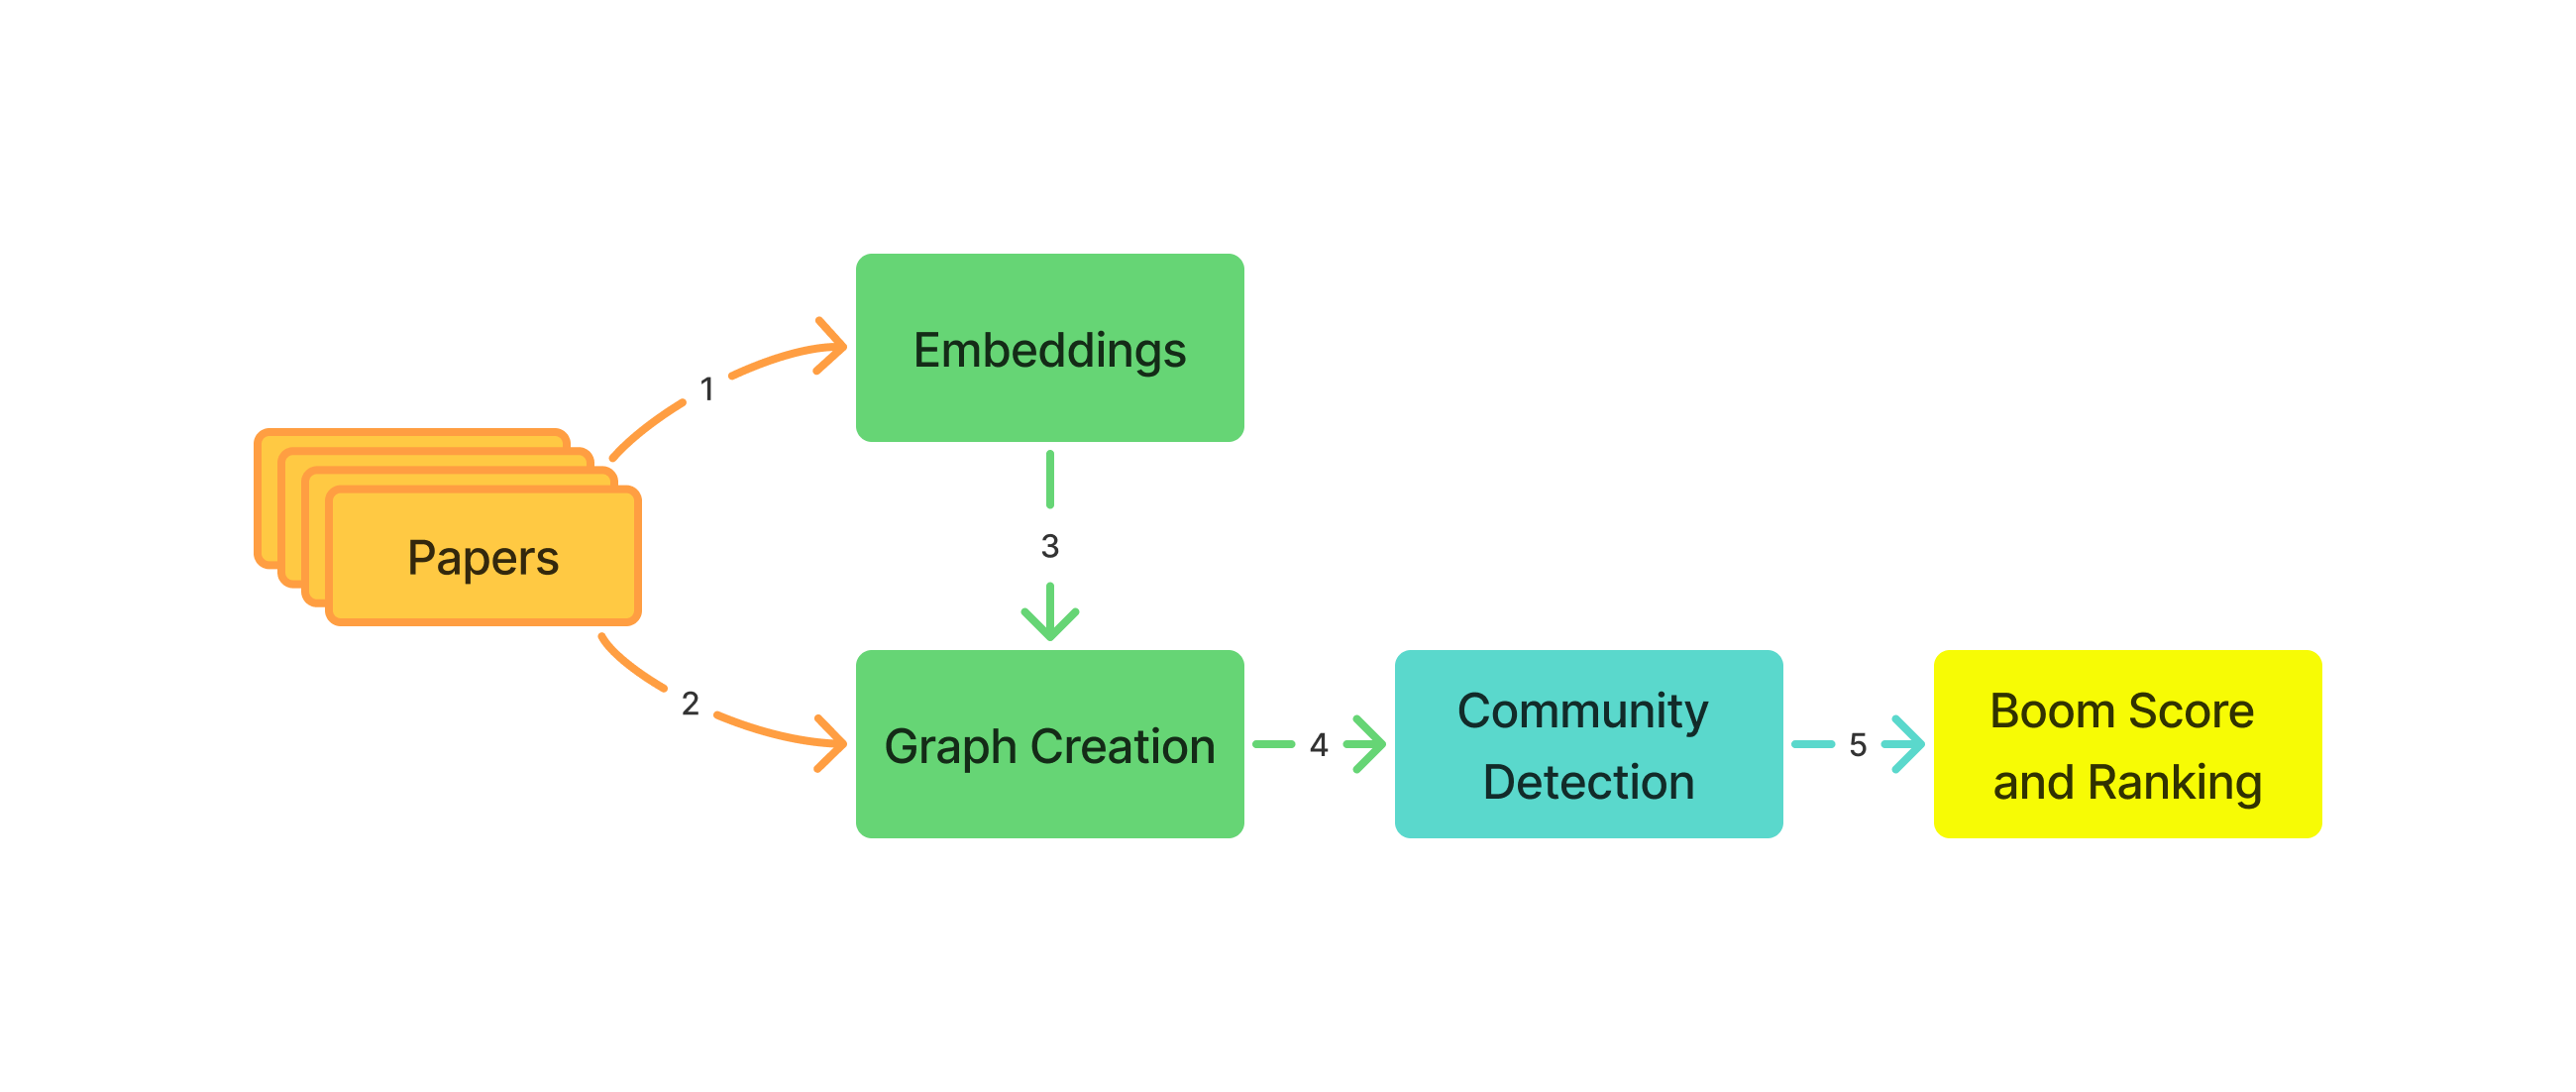
\includegraphics[width=15cm]{assets/systemflow.png}
    \caption{High-level System Architecture Overview}
\end{figure}

\subsection{Data Collection}

For the data collection phase, we will utilize the \textbf{OpenAlex}\parencite{openalex} dataset, a comprehensive and fully open bibliographic catalog of the global research ecosystem. OpenAlex is uniquely suited for our objective of discovering emerging communities in a graph because it provides a massive, interconnected web of scholarly entities and their relationships. By treating this data as a heterogeneous network, we can identify clusters of research activity as they form.

The following key attributes from OpenAlex will be extracted to construct the nodes and edges of our graph:
\vspace{-25pt}
\begin{enumerate}
    \item \textbf{Openalex ID} 
    \vspace{-10pt}
    \item \textbf{DOI} 
    \vspace{-10pt}
    \item \textbf{title}
    \vspace{-10pt}
    \item \textbf{publication date}
    \vspace{-10pt}
    \item \textbf{authorships}
    \vspace{-10pt}
    \item \textbf{fwci}
    \vspace{-10pt}
    \item \textbf{cited by count}
    \vspace{-10pt}
    \item \textbf{topics}
    \vspace{-10pt}
    \item \textbf{referenced works}
    \vspace{-10pt}
    \item \textbf{inverted index of Abstract}
\end{enumerate}

\subsection{Graph Construction}
This graph will be implemented using NetworkX\parencite{networkx} for rapid prototyping and 
small-scale analysis or igraph\parencite{igraph} for handling larger datasets with efficient 
querying capabilities and effective implementation of foundational traditional community 
detection algorithms. Gephi will be used for visualizing the graph structure and community 
clusters, providing insights into the overall topology and emerging patterns. 
\subsubsection{Citation Graph}
The citation graph represents papers as nodes and citation links as directed edges,
where an edge from Paper A to Paper B indicates that A cites B. 
\begin{figure}[H]
    \centering
    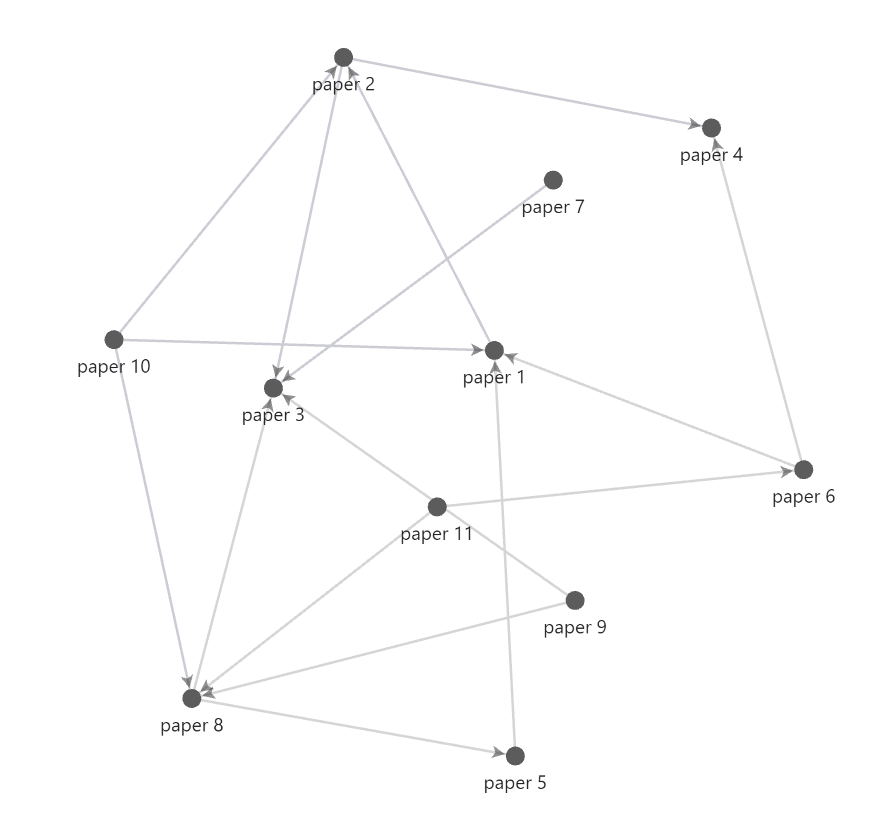
\includegraphics[width=5cm]{assets/citationgraph.png}
    \caption{Example citation graph with dummy nodes}
\end{figure}

\subsubsection{Paper-Author Graphs}
Paper-Author Graphs will extend the citation graph by incorporating additional
author information: author networks (edges between co-authors and edges from papers 
to their authors). This multi-layered graph provides a holistic view of academic 
connections, enabling more nuanced retrieval by linking papers through authors and 
beyond direct citations.
\begin{figure}[H]
    \centering
    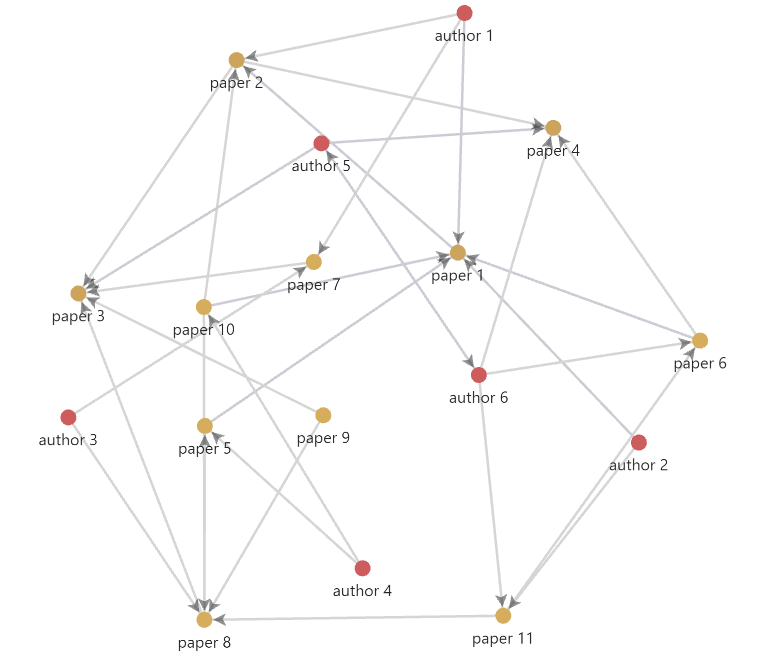
\includegraphics[width=5cm]{assets/paperauthorgraph.png}
    \caption{Example paper author graph with dummy nodes}
\end{figure}

\subsection{Community Detection}
To identify emerging research communities, we will apply a combination of traditional 
and advanced community detection algorithms. Traditional methods such as 
Leiden\parencite{traag_louvain_2019} and Infomap\parencite{smiljanic_community_2023} will be 
used to establish baseline community structures based on modularity optimization. These 
algorithms will help us understand the initial clustering of papers based on citation patterns.  

\subsection{Topic Extraction}
After communities have been identified every community will be assigned a topic
as a aggregated vote from all nodes in the community. The topics from each paper
will be extracted using BertTopic\parencite{grootendorst_bertopic_2022} or KeyBert\parencite{issa_comparative_2023}.

\subsection{Embeddings}
\subsubsection{Semantic Embeddings of Papers}
Semantic representations will be generated for the text of each paper (title and abstract) 
to fully capture its content and context. SciBERT\parencite{beltagy_scibert_2019}, a 
transformer model fine-tuned on scientific texts, will process the full text in segments 
(e.g., 512-token chunks) due to its input constraints, producing contextual embeddings 
(768-dimensional vectors) for each segment. These will be averaged across segments to create 
a single content-based embedding per paper, reflecting its scientific meaning. 

\subsubsection{Embeddings of Authors}
Author embeddings will be generated by aggregating the embeddings of their published papers, 
their researcher statistics like H-index, and their co-authorship network features. This 
will create a comprehensive representation of each author's influence and research focus.

We may also use a densely connected feedforward neural network to further refine the author 
embeddings.

\subsubsection{Graph-Based Embeddings}
After obtaining the SciBERT embeddings, we will use node2vec\parencite{grover_node2vec_2016} 
to further transform the embeddings to include the structural nuances. This will serve as our 
baseline for the graph-based models, capturing both the semantic content and the structural 
position of each paper within the citation network.

For GNNs, we will utilize the foundational GCN\parencite{kipf_semi-supervised_2016} and DrGNN 
architecture\parencite{zhang_gresnet_2019} to create a unified representation that 
integrates both the semantic and structural dynamics of research communities. 

\subsection{The Ranking of Communities}
For the ranking of communities, we will compute a \textbf{"Boom Score"} for each community using dense neural layers. Rather than predicting a fixed growth value, the model will be trained using a \textbf{Learning to Rank (LTR)} strategy. This approach focuses on the relative potential of communities, identifying which topics are likely to outperform others within the same academic domain.

\subsubsection{Training Loop}
The model will be trained using a \textbf{Pairwise Ranking} objective, specifically a RankNet-inspired framework, to optimize the structural and semantic ordering of communities:
\vspace{-25pt}
\begin{itemize}
    \item \textbf{Input Representation:} Each community $C_i$ is represented by a feature vector $x_i$ that concatenates structural graph metrics (from Leiden/Infomap) with semantic embeddings (from BERTopic).
    \item \textbf{Pairwise Objective:} During training, the model $f_\theta$ processes pairs of communities $(C_i, C_j)$ sampled from the same time snapshot. If Community $C_i$ historically showed higher citation growth in subsequent OpenAlex snapshots than $C_j$, the model is penalized if $f_\theta(x_i) < f_\theta(x_j)$.
    \item \textbf{Optimization:} We utilize a \textbf{Binary Cross-Entropy loss} over the score differences, forcing the model to maximize the margin between "booming" and "stable" communities. 
\end{itemize}
\vspace{-20pt}
By adopting a ranking-based approach, the framework remains robust to the high variance in citation scales across different scientific fields, ensuring that "breakout" topics are prioritized regardless of their niche.
\newpage

\section{System Requirement Specification}
\subsection{Software Specifications}
\subsubsection{Front-End Techologies}
\begin{itemize}
    \item Core UI Library: React.js
    \vspace{-10pt}
    \item Next.js (React Framework)
    \vspace{-10pt}
    \item Plotly (for interactive visualizations)
\end{itemize}

\subsubsection{Back-End Techologies}
\begin{itemize}
    \item Python (primary programming language)
    \vspace{-10pt}
    \item FastAPI (for building scalable and high-performance APIs)
\end{itemize}

\subsubsection{Database Systems}
\begin{itemize}
    \item Faiss Vector Database
    \vspace{-10pt}
    \item Neo4j Graph Database
\end{itemize}

\subsubsection{Machine Learning and AI Frameworks}
\begin{itemize}
    \item PyTorch (for training and fine-tuning deep learning models)
    \vspace{-10pt}
    \item Pytorch Geometric (for GNNs)
    \vspace{-10pt}
    \item igraph (for graph analysis)
\end{itemize}

\subsection{Hardware Specifications}
\subsubsection{Minimum Hardware Requirements}
\begin{itemize}
    \item Processor: Intel Core i7 (or equivalent) with at least 8 cores
    \vspace{-10pt}
    \item RAM: 16GB (recommended: 32GB for handling large embeddings)
    \vspace{-10pt}
    \item Storage: SSD with at least 1TB (recommended: NVMe SSD for fast retrieval)
    \vspace{-10pt}
    \item GPU: NVIDIA RTX 3060 (or higher) for model inference and training
\end{itemize}
\newpage

\section{Project Planning and Scheduling}
\begin{figure}[H]
\centering
\resizebox{\textwidth}{!}{%
\begin{ganttchart}[
    hgrid,
    vgrid,
    x unit=1.0cm,
    y unit title=0.5cm,
    y unit chart=0.45cm,
    title height=1,
    bar height=0.6,
    group height=0.3,
    bar/.append style={fill=blue!40},
    group/.append style={fill=gray!50},
    title label font=\scriptsize,
    bar label font=\scriptsize,
    group label font=\scriptsize\bfseries,
    canvas/.append style={draw=black},
]{1}{16}

\gantttitle{Project Timeline (16 Weeks)}{16} \\
\gantttitlelist{1,...,16}{1} \\

\ganttgroup{Phase 1}{1}{3} \\
\ganttbar{Literature Review}{1}{2} \\
\ganttbar{Boom Score Formulation}{1}{2} \\
\ganttbar{Data Collection}{3}{3} \\

\ganttgroup{Phase 2}{4}{5} \\
\ganttbar{Data Cleaning}{4}{4} \\
\ganttbar{Feature Engineering}{5}{5} \\

\ganttgroup{Phase 3}{6}{7} \\
\ganttbar{Citation Graph + Snapshots}{6}{6} \\
\ganttbar{Heterogeneous Graph}{7}{7} \\

\ganttgroup{Phase 4}{8}{13} \\
\ganttbar{Community Detection}{8}{9} \\
\ganttbar{Graph Embeddings}{10}{11} \\
\ganttbar{Boom Score Training}{12}{12} \\
\ganttbar{Hyperparameter Tuning}{13}{13} \\

\ganttgroup{Phase 5}{14}{16} \\
\ganttbar{Compile Results}{14}{14} \\
\ganttbar{Evaluation \& Analysis}{15}{15} \\
\ganttbar{Final Documentation}{16}{16} \\

\ganttbar[bar/.append style={fill=green!40}]{Documentation (ongoing)}{1}{16} \\

\end{ganttchart}%
}
\caption[Project Gantt Chart]{Project Gantt Chart --- EmerG-Net development timeline
across 16 weeks. Color coding:
\textcolor{gray}{$\blacksquare$} Phase groups,
\textcolor{blue!60}{$\blacksquare$} Task bars,
\textcolor{green!60}{$\blacksquare$} Ongoing documentation.}
\label{fig:gantt}
\end{figure}
\vspace{-35pt}
\noindent\textbf{Phase Descriptions:}
\vspace{-25pt}
\begin{itemize}
    \item \textbf{Phase 1 Foundation (Weeks 1--3):} Literature review and finalization 
    of the Boom Score formulation, followed by data collection via scholarly APIs 
    (OpenAlex).
    \vspace{-10pt}
    \item \textbf{Phase 2 Data Pipeline (Weeks 4--5):} Deep cleaning, deduplication, 
    and schema normalization of raw data, followed by feature engineering including 
    SciBERT embeddings, author statistics, and keyword extraction.
    \vspace{-10pt}
    \item \textbf{Phase 3 Graph Construction (Weeks 6--7):} Construction of temporal 
    citation graph snapshots and extension to a heterogeneous paper-author graph, 
    with structural validation.
    \vspace{-10pt}
    \item \textbf{Phase 4 Modeling and Experimentation (Weeks 8--13):} The core 
    experimental phase, covering community detection baselines (Leiden, Infomap), 
    graph embedding experiments (node2vec, GCN, DrGNN), Boom Score supervised training, 
    and hyperparameter tuning with ablation studies.
    \vspace{-10pt}
    \item \textbf{Phase 5 Results and Wrap-up (Weeks 14--16):} Compilation of results 
    and visualizations, evaluation and failure analysis, and final project documentation 
    and presentation preparation.
    \vspace{-10pt}
    \item \textbf{Documentation (Ongoing, Weeks 1--16):} Incremental documentation 
    maintained throughout all phases to avoid end-stage bottlenecks.
\end{itemize}

\newpage\section{Expected Outcome}
The expected outcome of this project is the development of a novel predictive metric, 
termed the “Boom Score,” designed to quantify the future impact potential of emerging 
research communities before they achieve widespread recognition. Unlike traditional 
retrospective indicators such as citation counts or H-index, the Boom Score will integrate 
multiple forward-looking signals, including temporal citation dynamics (awakening time), 
structural growth patterns within the graph, and semantic evolution of research topics. 
This metric aims to capture early-stage momentum and identify non-linear trends such as 
“Sleeping Beauty” phenomena, enabling the detection of high-potential research clusters 
at their formative stages.

In addition to the metric itself, the project will deliver a reusable and extensible 
framework for modeling and analyzing temporal heterogeneous graphs. This framework will 
unify semantic embeddings derived from transformer-based models with structural 
representations learned through graph-based techniques such as node2vec and Graph Neural 
Networks. Designed with modularity and scalability in mind, the system can be adapted 
beyond scholarly citation networks to other domains such as social media, innovation 
networks, and knowledge graphs. Together, the Boom Score and the supporting framework 
will provide a general-purpose tool for early trend detection, offering both practical 
utility and a foundation for future research in predictive graph analytics.

\newpage

\renewcommand{\refname}{\textit{References}} 
\addcontentsline{toc}{section}{\textit{References}}
\printbibliography
\newpage

\newpage

\end{document}
